\begin{figure*}[t!]
%\vspace*{-2ex}
\centering
%\setlength{\tabcolsep}{3pt} % Default value: 6pt
%\renewcommand{\arraystretch}{0.5} % Default value: 1
%
%\hspace*{-6ex}
%\begin{tabular}{ll}
%\hspace*{-6ex}
%\begin{tabular}{c} 
%\hspace*{-6ex}
%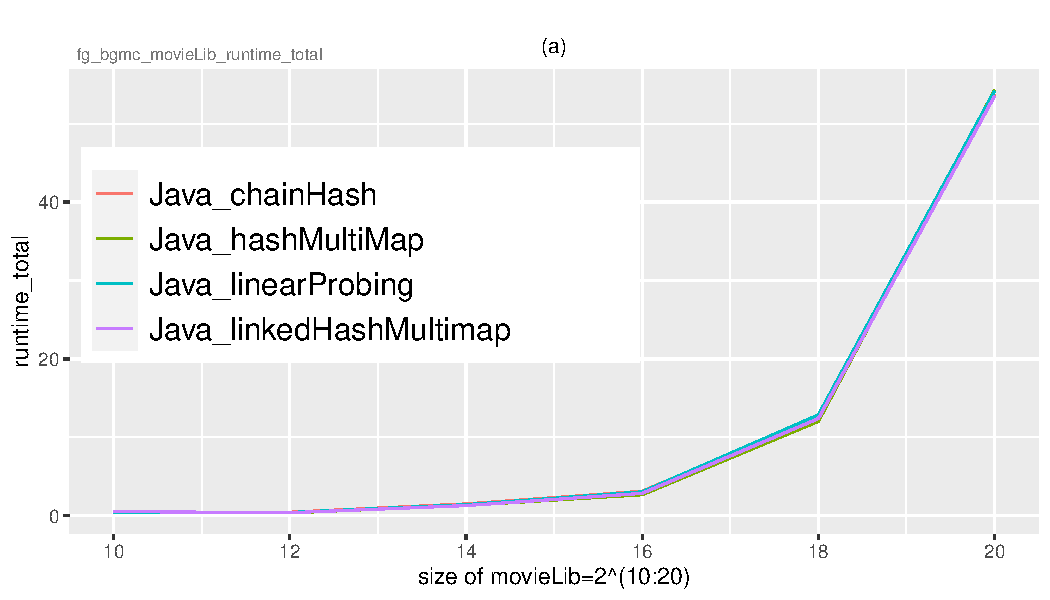
\includegraphics[width=0.45\textwidth]{../_Figures/fg_bgmc/fg_bgmc_movieLib_runtime_total_a}
%\end{tabular}
%
%&
%
%\begin{tabular}{c} 
%\hspace*{-6ex}
%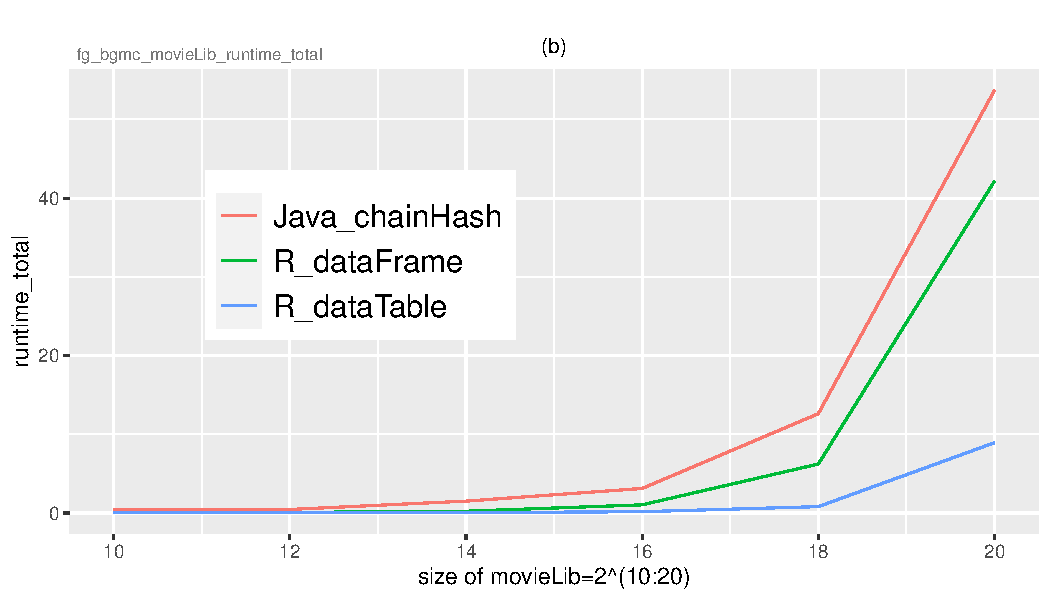
\includegraphics[width=0.45\textwidth]{../_Figures/fg_bgmc/fg_bgmc_movieLib_runtime_total_b}
%\end{tabular}
%
%\\[1ex]
%
%\begin{tabular}{c} 
%\hspace*{-6ex}
%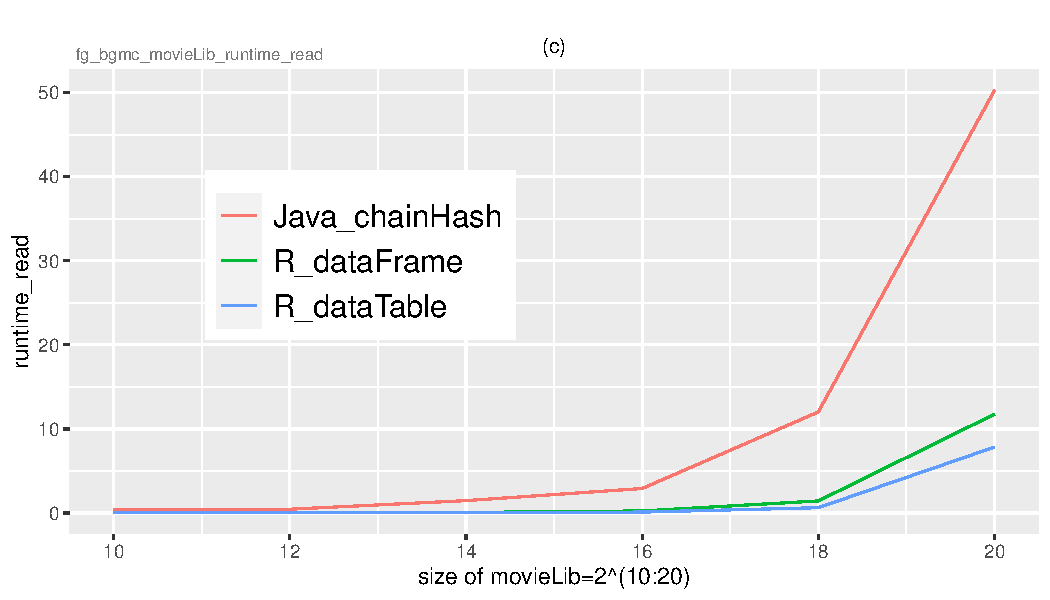
\includegraphics[width=0.45\textwidth]{../_Figures/fg_bgmc/fg_bgmc_movieLib_runtime_read_c}
%\end{tabular}
%
%&
%
%\begin{tabular}{c} 
%\hspace*{-6ex}
%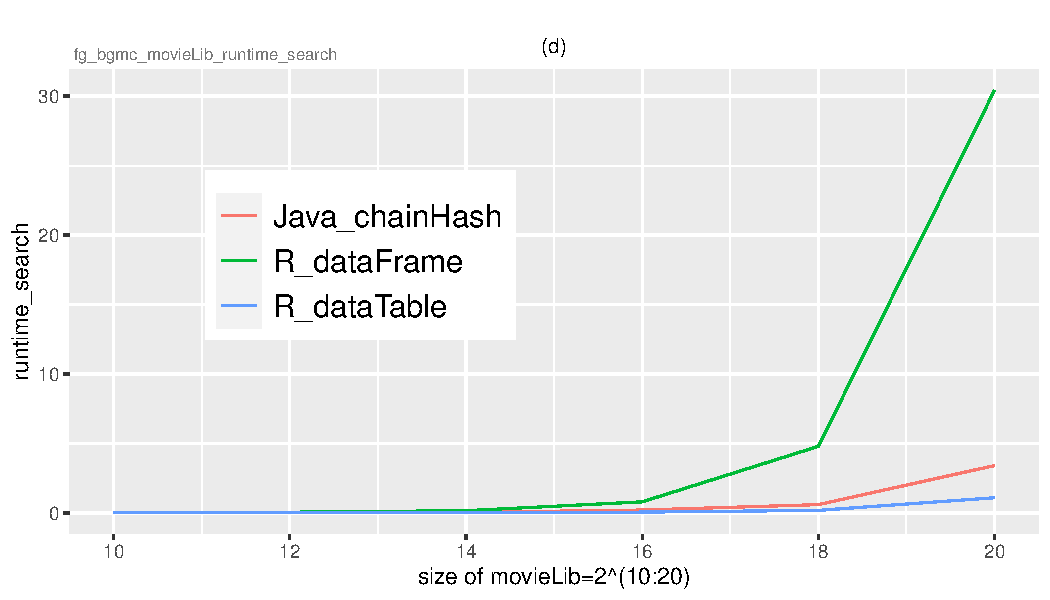
\includegraphics[width=0.45\textwidth]{../_Figures/fg_bgmc/fg_bgmc_movieLib_runtime_search_d}
%\end{tabular}
%
%\end{tabular} 

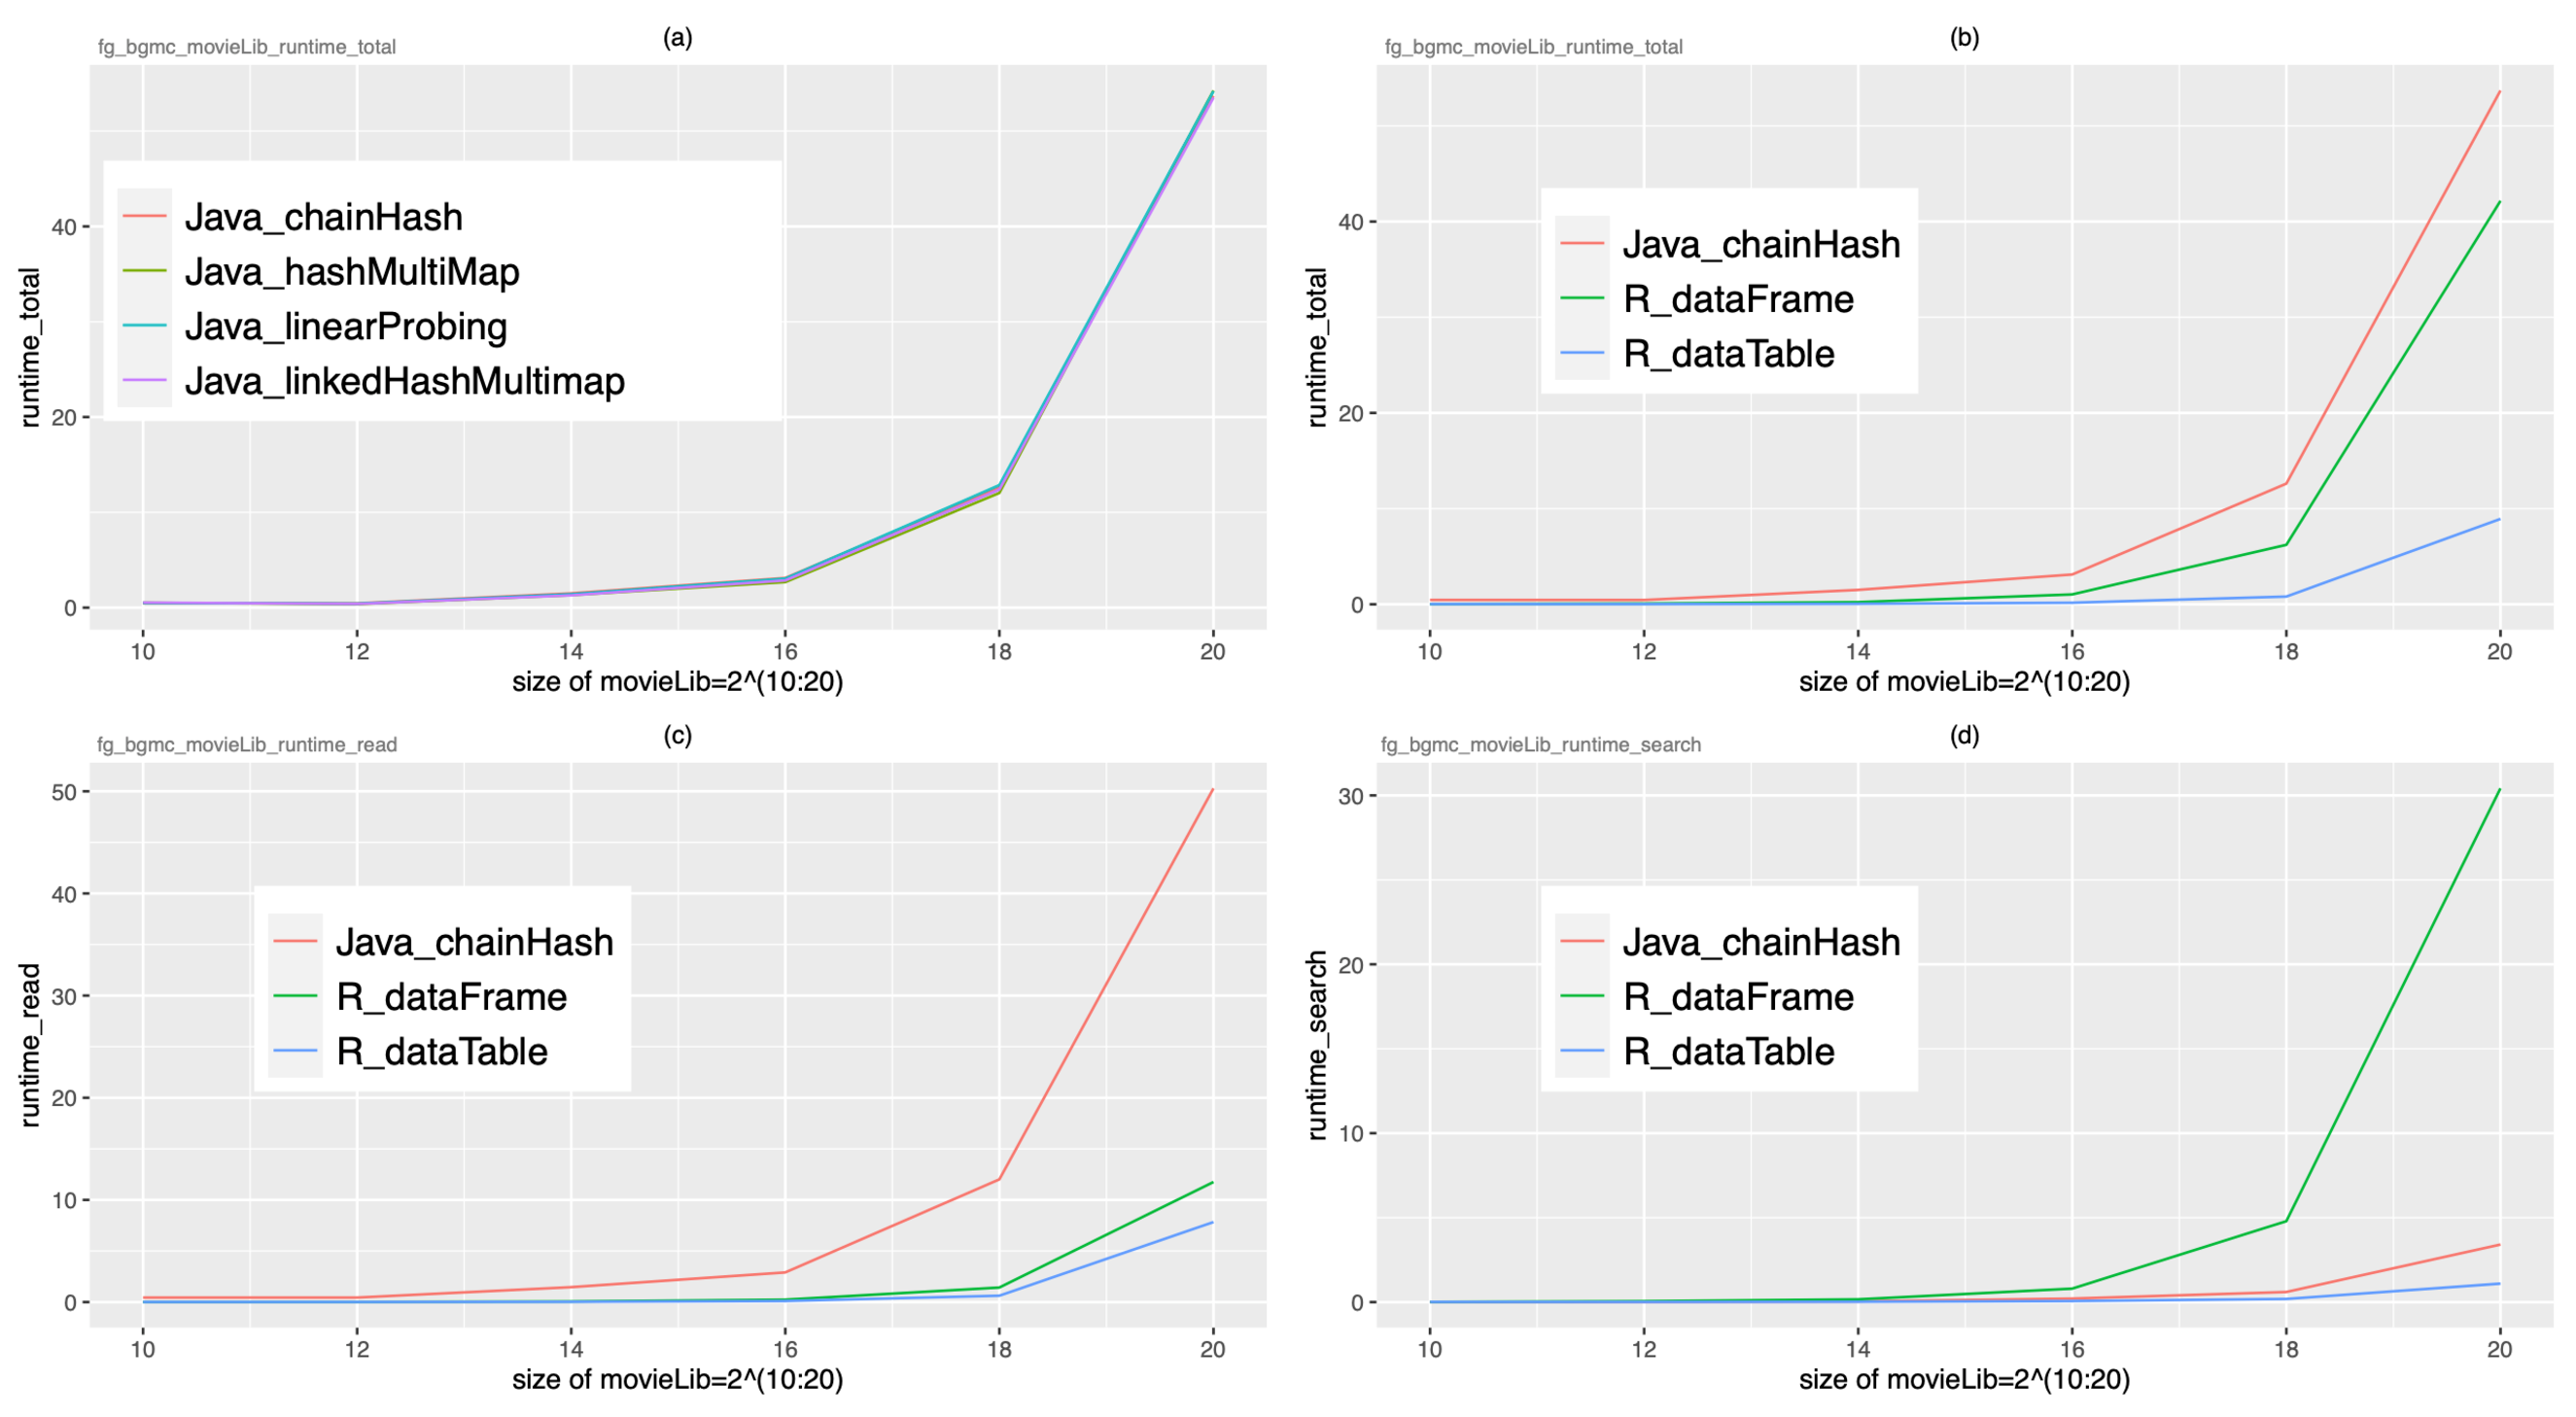
\includegraphics[width=1.0\textwidth]{_Figures/fg_bgmc_movieLib_runtime_abcd}

\caption{
Asymptotic runtime performance experiments with instances from {\it movieLib}, 
based on Java and R code. In each case, the objective is to retrieve the top 10
movies after reading two sets of files: one listing movies and one listing 
viewer interactions with each movie.
In (a), we report {\it runtime\_total} for best four data structures in Java; 
a model used in CSC316 class.
In (b), we report on {\it runtime\_total} for the single best data structure in Java ({\t chainHash}) in comparison with two best data structures in R ({\t dataFrame} and {\t dataTable}).
In (c), we report {\it runtime\_read} for {\it chainHash} in Java and {\it dataFrame} and {\it dataTable}
in R.
In (d), we report {\it runtime\_search} for {\it chainHash} in Java and {\it dataFrame} and {\it dataTable}
in R.
There is no doubt that, for  instances from {\it movieLib}, 
R significantly outperforms Java -- with {\it dataTable} an asymptotically better data structure in 
comparison with {\it dataFrame}.
}
\OMIT{
\caption{Experiments that analyze the total runtime, reading runtime and searching runtime for all Java and R programs. Data table version in R has a significantly improvement in runtime performance comparing to the others. The main obstacle that slows down the Java program is when reading data files and converting each line of information into an object. However, the Java program runs relatively fast when manipulating in the movieLib. Overall, the data table version of R program outperforms in any aspect including reading files and searching movies.}
}
\label{fg_bgmc_movieLib_runtime}
\end{figure*}
